% !TEX encoding = UTF-8 Unicode

\documentclass[aspectratio=169]{beamer}
\usepackage[utf8]{inputenc}

%% BIB
\usepackage[style=authoryear,backend=biber,url=false]{biblatex}
\addbibresource{nems.bib}
\addbibresource{yeast.bib}

%% GRAPHICS

\usepackage{graphicx}
\graphicspath{{images/}}
\usepackage{tikz}

%% COLORS
\definecolor{UWRed}{HTML}{C5050C}
\definecolor{StrongBlue}{HTML}{3F8FD2}
\definecolor{StrongGreen}{HTML}{36C88E}
\definecolor{StrongRed}{HTML}{9B0000}
\definecolor{MyC}{HTML}{009999}
\definecolor{MyM}{HTML}{990099}
\definecolor{MyY}{HTML}{999900}
\definecolor{MyR}{HTML}{990000}
\definecolor{MyG}{HTML}{009900}
\definecolor{MyB}{HTML}{000099}
\definecolor{ActionRed}{HTML}{990000}

%% SLIDE COLOR SETTINGS
\setbeamercolor{structure}{fg=UWRed}
\setbeamercolor{title page}{fg=white}
\setbeamercolor{title}{fg=white}

%% RM NAV SYMBOLS
\setbeamertemplate{navigation symbols}{}

%% FONTS
\setbeamerfont{title}{size=\huge\bfseries}

%% DRAWING
\usetikzlibrary{fit,calc,arrows,arrows.meta,decorations.pathreplacing,decorations.text,decorations.pathmorphing,backgrounds,fit,positioning,shapes,chains,topaths,matrix}

\def\firstcircle{(90:0.3cm) circle (0.6cm)}
\def\secondcircle{(210:0.3cm) circle (0.6cm)}
\def\thirdcircle{(330:0.3cm) circle (0.6cm)}

\tikzset{%
  link/.style={->,>=angle 45,semithick},
  var/.style={circle,draw,minimum size=1.5em,align=center, inner sep=0pt, anchor=center},
  text block/.style={rectangle, rounded corners, draw=#1, fill=white, thick, text width=5em, align=center},
  thick arrow/.style={
     -{Triangle[angle=120:1pt 1]},
%     -Triangle,
     line width=2em, 
     draw=SoftBlue
  },
  arrow label/.style={
    text=white,
    font=\sf,
    align=center
  },
  set mark/.style={
    insert path={
      node [midway, arrow label, node contents=#1]
    }
  },
  set vertical mark/.style={
    insert path={
      node [midway, arrow label, node contents=#1, rotate=-90]
    }
  },
  colormap/.pic={code={    
    \fill[MyC] \firstcircle;
    \fill[MyM] \secondcircle;
    \fill[MyY] \thirdcircle;
    
    % C+M, C+Y
    \begin{scope}
      \clip \firstcircle;
      \fill[MyB] \secondcircle;
      \fill[MyG] \thirdcircle;
    \end{scope}
    
    % M+Y, K
    \begin{scope}
      \clip \secondcircle;
      \fill[MyR] \thirdcircle;
      \clip \firstcircle;
      \fill[black] \thirdcircle;
    \end{scope}
    
    \draw[thick, white] \firstcircle;
    \draw[thick, white] \secondcircle;
    \draw[thick, white] \thirdcircle;
    
    \node[white] at (90:0.6cm) {\scriptsize\bf 1};
    \node[white] at (210:0.6cm) {\scriptsize\bf 2};
    \node[white] at (330:0.6cm) {\scriptsize\bf 3};
  }},
  onslide/.code args={<#1>#2}{
    \only<#1>{\pgfkeysalso{#2}}
  }
}

%% LOGO on slides
\logo{\begin{tikzpicture}[overlay]
  \node[anchor=north east,inner sep=0] at (0,86mm) {
\includegraphics[height=10mm]{SMPH_color-flush.pdf}};
\end{tikzpicture}}

%% CONTENT BEGINS

\title{Context-Specific Nested Effect Models}
\subtitle{RECOMB 2018}
\author{Yuriy Sverchkov}
\institute{University of Wisconsin--Madison}
\date{April 24, 2018}

\begin{document}

  {
    \usebackgroundtemplate{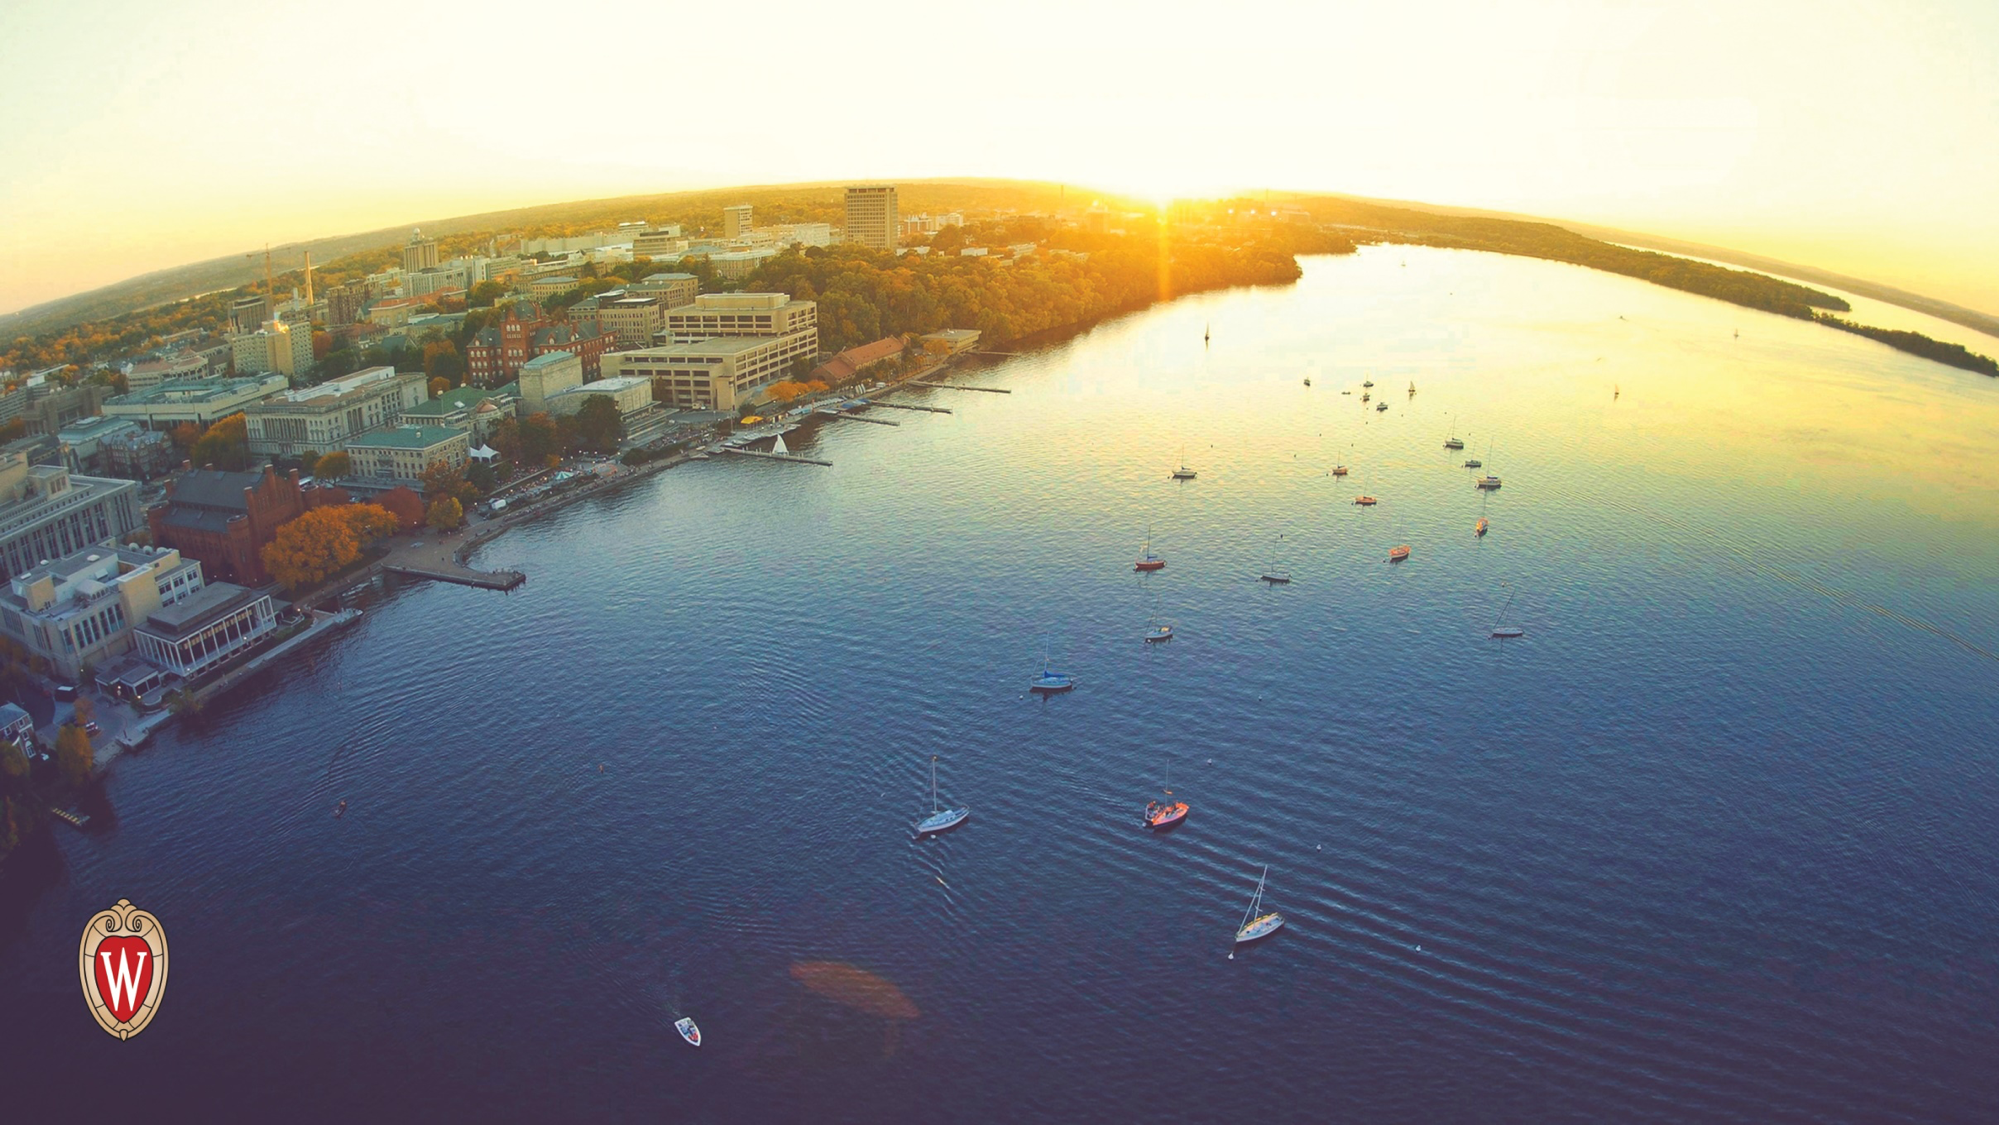
\includegraphics[width=\paperwidth]{UW-lake.png}}
    \begin{frame}[plain]
      \vskip4cm
      \titlepage
    \end{frame}
  }
  
  %%% FRAMEBREAK %%%

\begin{frame}{Uncovering biological networks}
  \centering
  \begin{tikzpicture}[very thick, ampersand replacement=\&]

    \matrix (es) [matrix of nodes, column sep = 0.5em] at (0,-2cm) {
      \& |[fill=StrongGreen,onslide={<4,5>{fill=StrongRed}}]|$e_1$
      \&  |[fill=StrongGreen,onslide={<4,5>{fill=StrongBlue}}]|$e_2$
      \& |[fill=StrongRed,onslide={<4,5>{fill=StrongBlue}}]|$e_3$
      \& |[fill=StrongRed,onslide={<4>{fill=StrongBlue}}]|$e_4$
      \& |[fill=StrongBlue]|$e_5$
      \& |[fill=StrongGreen,onslide={<4,6>{fill=StrongBlue}}]|$e_6$
      \& |[fill=StrongBlue,onslide={<4,6>{fill=StrongGreen}}]|$e_7$
      \& |[fill=StrongRed,onslide={<4,6>{fill=StrongGreen}}]|$e_8$ \\
    };

    \uncover<3->{
      \node[var] (a) at (0,0) {A};
      \node[var] (b) at (-1cm, -1cm) {B}; 
      \node[var] (c) at (1cm, -1cm) {C};

      \draw[link,onslide=<4>{ActionRed}] (a) to (b);
      \draw[link,onslide=<4>{ActionRed}] (a) to (c);
      \draw[link,{onslide=<4,5>{ActionRed}}] (b) to (es-1-2);
      \draw[link,{onslide=<4,5>{ActionRed}}] (b) to (es-1-3);
      \draw[link,{onslide=<4,5>{ActionRed}}] (b) to (es-1-4);
      \draw[link,onslide=<4>{ActionRed}] (a) to (es-1-5);
      \draw[link,{onslide=<4,6>{ActionRed}}] (c) to (es-1-7);
      \draw[link,{onslide=<4,6>{ActionRed}}] (c) to (es-1-8);
      \draw[link,{onslide=<4,6>{ActionRed}}] (c) to (es-1-9);
    }
    
    \only<4>{
      \draw[very thick, ActionRed] (a.north west) to (a.south east);
      \node[anchor=west, ActionRed] at (a.east) {$\Delta$};
    }
    \only<5>{
      \draw[very thick, ActionRed] (b.north west) to (b.south east);
      \node[anchor=west, ActionRed] at (b.east) {$\Delta$};
    }
    \only<6>{
      \draw[very thick, ActionRed] (c.north west) to (c.south east);
      \node[anchor=west, ActionRed] at (c.east) {$\Delta$};
    }
    
    \node[draw, ellipse, very thick, fit=(a) (b) (c) (es)] (cell) {};

  \matrix (d) [below=5mm of cell, matrix of nodes, nodes={}] {
  \& $e_1$ \& $e_2$ \& $e_3$ \& $e_4$ \& $e_5$ \& $e_6$ \&  $e_7$ \& $e_8$ \\
  WT \& |[fill=StrongGreen]| \&  |[fill=StrongGreen]| \& |[fill=StrongRed]| \& |[fill=StrongRed]| \& |[fill=StrongBlue]| \& |[fill=StrongGreen]| \& |[fill=StrongBlue]| \& |[fill=StrongRed]| \\
  $A\Delta$ \& |[fill=StrongRed]| \&  |[fill=StrongBlue]| \& |[fill=StrongBlue]| \& |[fill=StrongBlue]| \& |[fill=StrongBlue]| \& |[fill=StrongBlue]| \& |[fill=StrongGreen]| \& |[fill=StrongGreen]| \\
  $B\Delta$ \& |[fill=StrongRed]| \&  |[fill=StrongBlue]| \& |[fill=StrongBlue]| \& |[fill=StrongRed]| \& |[fill=StrongBlue]| \& |[fill=StrongGreen]| \& |[fill=StrongBlue]| \& |[fill=StrongRed]| \\
  $C\Delta$ \& |[fill=StrongGreen]| \&  |[fill=StrongGreen]| \& |[fill=StrongRed]| \& |[fill=StrongRed]| \& |[fill=StrongBlue]| \& |[fill=StrongBlue]| \& |[fill=StrongGreen]| \& |[fill=StrongGreen]| \\
 };
  \uncover<1>{ \node[fill=white,fit=(d-2-1) (d-1-9), inner sep=0] {};}
  \uncover<4->{ \node[fill=white,opacity=0.5, fit=(d-2-1) (d-2-9), inner sep=0] {};}
  \node[fill=white,onslide=<4>{opacity=0},onslide=<5-6>{opacity=0.5},fit=(d-3-1) (d-3-9), inner sep=0] {};
  \node[fill=white,onslide=<5>{opacity=0},onslide=<6>{opacity=0.5},fit=(d-4-1) (d-4-9), inner sep=0] {};
  \uncover<-5>{ \node[fill=white,fit=(d-5-1) (d-5-9), inner sep=0] {};}
  
 %   \uncover<7>{
 %     \node[anchor=south, fill=white] at (d.north) {High-dimensional phenotype};
 %   }
  \end{tikzpicture}
\end{frame}

%%% FRAMEBREAK

\begin{frame}{Context-specific networks}
\end{frame}

%%% FRAMEBREAK %%%

\begin{frame}{High-dimensional knockout screens}

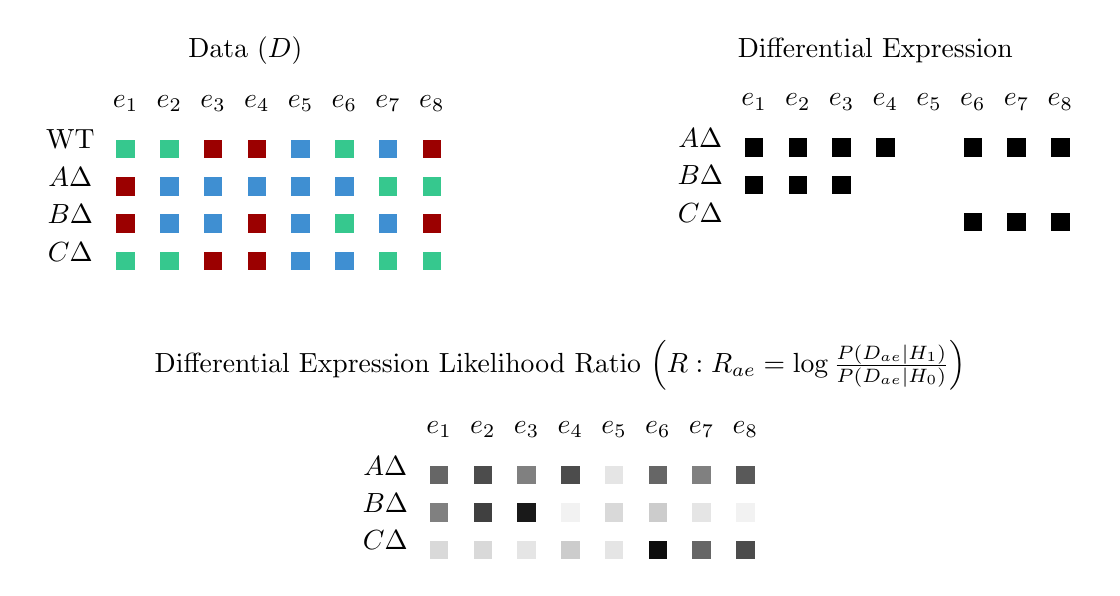
\begin{tikzpicture}[very thick, ampersand replacement=\&]

 \node (data) {Data ($D$)};
 \matrix (dmx) [anchor=north, matrix of nodes] at (data.south) {
  \& $e_1$ \& $e_2$ \& $e_3$ \& $e_4$ \& $e_5$ \& $e_6$ \&  $e_7$ \& $e_8$ \\
  WT \& |[fill=StrongGreen]| \&  |[fill=StrongGreen]| \& |[fill=StrongRed]| \& |[fill=StrongRed]| \& |[fill=StrongBlue]| \& |[fill=StrongGreen]| \& |[fill=StrongBlue]| \& |[fill=StrongRed]| \\
  $A\Delta$ \& |[fill=StrongRed]| \&  |[fill=StrongBlue]| \& |[fill=StrongBlue]| \& |[fill=StrongBlue]| \& |[fill=StrongBlue]| \& |[fill=StrongBlue]| \& |[fill=StrongGreen]| \& |[fill=StrongGreen]| \\
  $B\Delta$ \& |[fill=StrongRed]| \&  |[fill=StrongBlue]| \& |[fill=StrongBlue]| \& |[fill=StrongRed]| \& |[fill=StrongBlue]| \& |[fill=StrongGreen]| \& |[fill=StrongBlue]| \& |[fill=StrongRed]| \\
  $C\Delta$ \& |[fill=StrongGreen]| \&  |[fill=StrongGreen]| \& |[fill=StrongRed]| \& |[fill=StrongRed]| \& |[fill=StrongBlue]| \& |[fill=StrongBlue]| \& |[fill=StrongGreen]| \& |[fill=StrongGreen]| \\
  };
 \uncover<2->{
	\node (de) at (8,0) {Differential Expression};
	\matrix (demx) [anchor=north, matrix of nodes] at (de.south) {
  \& $e_1$ \& $e_2$ \& $e_3$ \& $e_4$ \& $e_5$ \& $e_6$ \&  $e_7$ \& $e_8$ \\
  $A\Delta$ \& |[fill=black]| \&  |[fill=black]| \& |[fill=black]| \& |[fill=black]| \& \& |[fill=black]| \& |[fill=black]| \& |[fill=black]| \\
  $B\Delta$ \& |[fill=black]| \& |[fill=black]| \& |[fill=black]| \& \& \& \& \& \& \& \& \\
  $C\Delta$ \& \& \& \& \& \& |[fill=black]| \& |[fill=black]| \& |[fill=black]| \\
 };
 }
 \uncover<3->{
	\node (lode) at (4,-4) {Differential Expression Likelihood Ratio $\left( R : R_{ae} = \log \frac{ \mathbb P( D_{ae} | H_1 ) }{ \mathbb P( D_{ae} | H_0 ) } \right)$};
	\matrix (lodemx) [anchor=north, matrix of nodes] at (lode.south) {
  \& $e_1$ \& $e_2$ \& $e_3$ \& $e_4$ \& $e_5$ \& $e_6$ \&  $e_7$ \& $e_8$ \\
  $A\Delta$ \& |[fill=black!60]| \&  |[fill=black!70]| \& |[fill=black!50]| \& |[fill=black!70]| \& |[fill=black!10]| \& |[fill=black!60]| \& |[fill=black!50]| \& |[fill=black!65]| \\
  $B\Delta$ \& |[fill=black!50]| \& |[fill=black!75]| \& |[fill=black!90]| \& |[fill=black!5]| \& |[fill=black!15]| \& |[fill=black!20]| \& |[fill=black!10]| \& |[fill=black!5]| \\
  $C\Delta$ \& |[fill=black!15]| \& |[fill=black!15]| \& |[fill=black!10]| \& |[fill=black!20]| \& |[fill=black!10]| \& |[fill=black!95]| \& |[fill=black!60]| \& |[fill=black!70]| \\
 };
 }
\end{tikzpicture}

\end{frame}

%%% FRAMEBREAK %%%

\begin{frame}{Nested effect model (NEM)}

\begin{columns}
\column{0.5\textwidth}

\begin{tikzpicture}[very thick, ampersand replacement=\&]

 {\color{StrongGreen}
  \matrix (es) [anchor=north, matrix of nodes] at (de.south) {
  \& $e_1$ \& $e_2$ \& $e_3$ \& $e_4$ \& $e_5$ \& $e_6$ \&  $e_7$ \& $e_8$ \\
  $A\Delta$ \& |[fill]| \&  |[fill]| \& |[fill]| \& |[fill]| \& \& |[fill]| \& |[fill]| \& |[fill]| \\
  $B\Delta$ \& |[fill]| \& |[fill]| \& |[fill]| \& \& \& \& \& \& \& \& \\
  $C\Delta$ \& \& \& \& \& \& |[fill]| \& |[fill]| \& |[fill]| \\
 };
  \node[anchor=north] at (es.south) {Effect matrix $F$};
 }
 
 \node[var, above=3 of es] (a) {A};
 \node[var, below left=of a] (b) {B}; 
 \node[var, below right=of a] (c) {C};
 
 {\color{StrongBlue}
 \draw[link] (a) to (b);
 \draw[link] (a) to (c);
 }
 {\color{StrongRed}
 \draw[link] (b) to (es-1-2);
 \draw[link] (b) to (es-1-3);
 \draw[link] (b) to (es-1-4);
 \draw[link] (a) to (es-1-5);
 \draw[link] (c) to (es-1-7);
 \draw[link] (c) to (es-1-8);
 \draw[link] (c) to (es-1-9);
 }

\end{tikzpicture}
\pause
\column{0.4\textwidth}

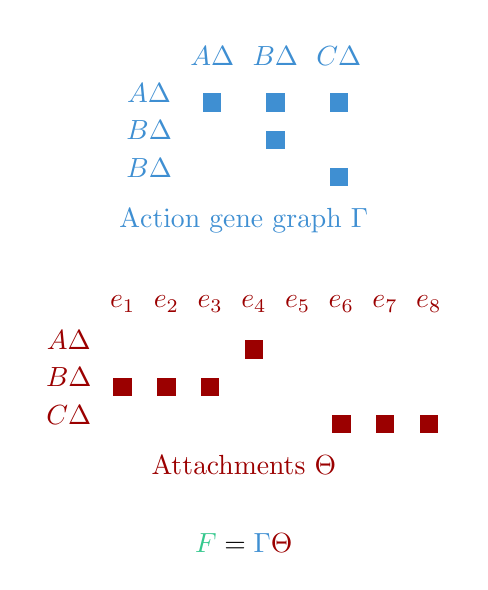
\begin{tikzpicture}[very thick, ampersand replacement=\&]

 {\color{StrongBlue} 
 \matrix (gamma) [matrix of nodes] {
  \& $A\Delta$ \& $B\Delta$ \& $C\Delta$ \\
  $A\Delta$ \& |[fill]| \&  |[fill]| \& |[fill]| \\
  $B\Delta$ \& \& |[fill]| \& \\
  $B\Delta$ \& \& \&  |[fill]| \\
 };
 \node[anchor=north] at (gamma.south) {Action gene graph $\Gamma$};
 }
 
 {\color{StrongRed}
 \matrix (theta) [below=of gamma, matrix of nodes] {
  \& $e_1$ \& $e_2$ \& $e_3$ \& $e_4$ \& $e_5$ \& $e_6$ \&  $e_7$ \& $e_8$ \\
  $A\Delta$ \& \& \& \& |[fill]| \& \& \& \& \\
  $B\Delta$ \& |[fill]| \& |[fill]| \& |[fill]| \& \& \& \& \& \& \& \& \\
  $C\Delta$ \& \& \& \& \& \& |[fill]| \& |[fill]| \& |[fill]| \\
 };
 \node[anchor=north] at (theta.south) {Attachments $\Theta$};
 }
 
 \node (formula) [below=of theta] {${\color{StrongGreen} F} = {\color{StrongBlue} \Gamma} {\color{StrongRed}\Theta}$};

\end{tikzpicture}

\end{columns}

{\tiny \parencite{Markowetz01012005}} %TODO: Add more
\end{frame}

%%% FRAMEBREAK %%%

\end{document}